
\documentclass{funthesis}

\usepackage{graphicx} % 図(EPS形式)を本文中で読み込む場合はこれを宣言
\usepackage{multirow}
%--------------------------------------------------------------------
\jtitle{DDoS攻撃を行うマルウェアのIoTデバイス本体\\における検知手法の提案}  % 論文の和文タイトル
%
\etitle{Mechanism on IoT device for Identifying Malicious Process}% 論文の英文タイトル
%
\htitle{Detection Method of DDos Attack}   % ヘッダー用の論文の短縮英文タイトル
%     必ず1行に収まるように英文タイトルを短縮する.
%
\jauthor{水上 敬介}    % 氏名(日本語)
\eauthor{Keisuke Mizukami}   % 氏名(英語)
\jaffiliciation{情報アーキテクチャ学科} % 所属学科名(日本語)
\eaffiliciation{Department of Information Architecture} % 所属学科名(英語)
\studentnumber{1015237}   % 学籍番号
\jadvisor{稲村 浩}    % 正指導教員名(日本語)
\jcoadvisor{中村 義隆} % 副指導教員(日本語)がいる場合は
                        % コメントアウトし名前を書く
                        % 副指導教員がいない場合は,ここは削除しても可
\eadvisor{Hiroshi. Inamura}  % 正指導教員名(英語)
\ecoadvisor{Yoshitaka. Nakamura}   % 副指導教員(英語)がいる場合は
                         % コメントアウトし名前を書く
                         % 副指導教員がいない場合は,ここは削除しても可
\jdate{2019年1月29日}    % 論文提出日   (日本語)
\edate{January 29, 2019}     % 論文提出年月 (英語)
% タイトルなどの定義の終わり

%--------------------------------------------------------------------

%-------------------------------------------------------------------
\begin{document}
\maketitle    % タイトルページを作成
%--------------------------------------------------------------------
% 英文概要(250語程度)
\begin{eabstract}
{In recent years, IoT devices equipped with communication functions in various things are spreading explosively. As a result It is a social problem that a botnet is constructed by an IoT device infected with malware and a DDoS attack is performed. Malware called Mirai is published on the web site, and many variants of Mirai are made. In this research, we aim to detect malware that performs DDoS attack on IoT device , and to detect unknown malware. we pay attention to the fact that the variants of malware were make from published malware on web site, we detect malware that performs DDoS attack by determining whether there is a specific function of the original malware}
\end{eabstract}

% 英文キーワード(5個程度をコンマ(,)で区切って羅列する)
\begin{ekeyword}
DDoS attack, IoT Device, malware, Mirai, Linux
\end{ekeyword}

%--------------------------------------------------------------------
% 和文概要(400字程度)
\begin{jabstract}
近年,世の中にある様々なものに通信機能を搭載したIoT機器が爆発的に普及している.その結果,マルウェアに感染したIoT機器によってボットネットが構築され大規模なDDoS攻撃が行われ大きな問題となっている.その中でも,Miraiと呼ばれるマルウェアがWeb上で公開され,Miraiの亜種が多く作られている.本研究では,IoTデバイス本体においてDDoS攻撃を行うマルウェアを検知する手法を検討することによって,未知のマルウェアでも検知を行えることを目的とする.公開されているマルウェアを元に亜種が作成されていることに着目をして,オリジナルのマルウェアが持つ特定の関数の挙動を検出することによってDDoS攻撃を行うマルウェアの検知を行う.
\end{jabstract}

% 和文キーワード(5個程度をコンマ(,)で区切って羅列する)
\begin{jkeyword}
DDoS攻撃,IoTデバイス,マルウェア,Mirai,Linux
\end{jkeyword}
\tableofcontents % 目次を作成
 %概要
\chapter{序論} % 章のタイトル

% \includegraphics[width=??cm]{hoge.eps} % 図(EPS形式)を読み込む場合

\section{背景} % sectionのタイトル

% 以下に背景,関連する環境状況,技術に関する概要を記述.

近年,インターネット技術やセンサー技術の進化を背景に,パソコンやスマートフォンなどのインターネット端末に加え,家電や自動車などの様々なものに通信機能を搭載したIoTデバイスが普及し始めている.総務省によると政界中のIoTデバイスの数は図1のように2017年時点でIoTデバイスが約275億台存在し,2020年にはIoTデバイスが403億台に及ぶと予想されている\cite{IoT}.
 \begin{figure}[h]
 \centering
    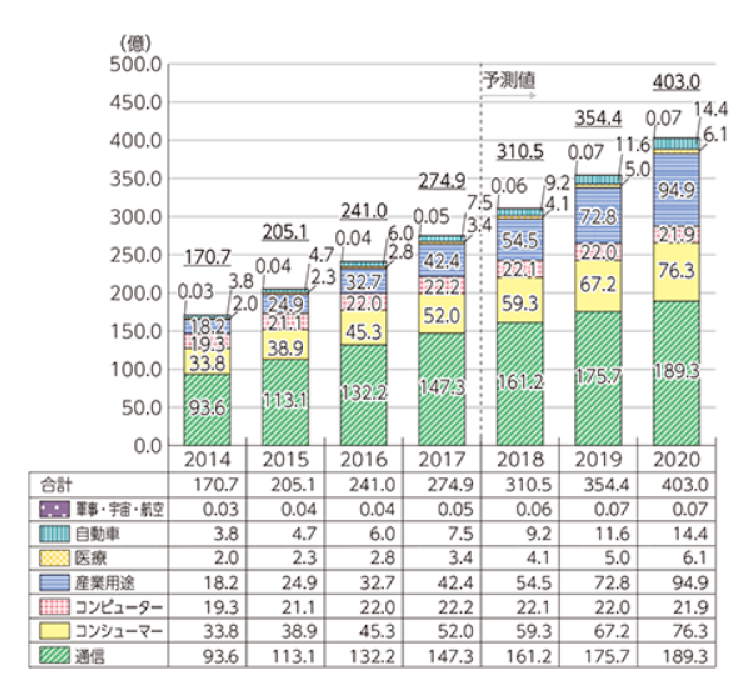
\includegraphics{figures/IoT_device.eps}
    \caption{世界のIoTデバイス数の推移及び予測}
 \label{fi:IoT}
 
 \end{figure}
%参考文献をしっかり入れ直す
IoTデバイスの普及に伴い,IoTデバイスを対象としたマルウェアが急増している.
IoTデバイスの重要な問題の1つとしてセキュリティ問題が挙げられる.IoTデバイスのユーザ名やパスワードを初期設定の状態で使用する場合が多いことやデバイスの資源が限られていることから,セキュリティが十分に考慮されていない事がある.そのため,IoTデバイスを対象としたマルウェアが脅威となっている.その中でもネットワークサービスを停止させる深刻な問題を引き起こしているマルウェアにはDDoS(Distributed Denial of Service)攻撃を行っているものが多く存在し,その対策が重要視されている.DDoS攻撃は,攻撃者が複数の他人のコンピュータを利用し,公開されているサービスに大量のデータを送りつける事によって処理負荷を与えサービスを機能停止に追い込む攻撃である.代表的なDDoS攻撃を行うマルウェアとしてMiraiが挙げられる.Mirai\cite{Mirai}は,無作為なIPアドレスから感染できるデバイスを探し出し,ログイン可能なデバイス上に,悪意のあるソフトウェアをダウンロードし実行させることでそのデバイスを制御下に置く.攻撃者によって制御された端末は他に侵入可能な端末を探し出し,次々と感染させることでボットネットと呼ばれる悪意あるプログラムを使用して乗っ取った多数のコンピュータで構成されるネットワークを構築する.その後,C\&C(Command and Control)サーバから送られた指示に対してDDoS攻撃を行うマルウェアである.2016年10月に発生した,DNSサーバープロバイダであるDyn社へのDDoS攻撃ではIoTデバイスによるボットネットが利用され史上最大規模である620Gbpsの攻撃が観測された\cite{Dyn}.その後,Miraiのソースコードが公開され,Owari,Satori,OkiruといったMiraiの亜種の開発が盛んに行われるようになった.2017年には,Windows PCを踏み台にして感染可能なIoTデバイスを探索するMiraiが観測された\cite{newMirai}.このMiraiはDoS攻撃を行う機能を有していないが,探索後にログイン可能な端末がLinuxデバイスであればDoS攻撃機能を有したMiraiをダウンロードさせ,Windows PCであればスキャン機能に特化したMiraiをダウンロードさせ,さらなるMiraiを様々なIoTデバイス拡散することが可能になっている.MiraiやMirai亜種のマルウェアによって,多くのIoTデバイスがDDoS攻撃に不正利用されるようになったことから,国立研究開発法人情報通信研究機構がパスワード設定などに不備のあるIoT機器の実態把握を目的として日本国内のIPv4アドレスを対象にSSH,Telnet,HTTPであるTCPの22番,23番,80番ポートを対象にポートスキャンを行った\cite{国立}.
%ここ少しおかしいから治す
IoTデバイスの不正利用によるDDoS攻撃が社会的に注目されている.

\section{IoTデバイスで検知を行う必要性}

IDS(Instrusion Detection System)と呼ばれるマルウェアによる不正な通信やホストへの侵入,ファイルの改ざん等の不正な挙動の兆候を検出するシステムの設置場所として2種類が考えられる.ネットワーク上に設置するネットワーク型と端末上に設置するホスト型の2種類が考えられる.ネットワーク型のIDSでは,ネットワークに流れるデータを取得して解析し,異常がないか確認する.不正が疑わ得れるデータを検知したときには管理者に知らせる.ネットワーク上でネットワークトラフィックからDDoS攻撃を判別するのは難しく誤検知する可能性が考えられる.しかし,マルウェアに基づいて作成されたデータを用いたパターンマッチングによる検知手法では,誤検知率が低く既存のマルウェアを確実に検知できる利点が有る.公開されているソースコードを基に作成されたマルウェアは,オリジナルのマルウェアと共通するシグネチャが存在すると考えられるためパターンマッチングによる検知で亜種のマルウェアにも対応できると想定される.脅威となっているマルウェアは,十分に管理が行われていないIoTデバイスで散見される,放置された初期パスワードのままのアカウントや,保守されていないシステムの脆弱性をついた攻撃を行うため,侵入されてしまうことは前提とすべきである.そのため,デバイスの性能が限られているIoTデバイス上でもマルウェアの検知を行う必要がある.

\section{マルウェアMiraiの概要}

Miraiは,ネットワーク上で公開されているLinuxで動作するデバイスを不正利用し,DDoS攻撃を行うマルウェアである.ネットワークカメラやルータといったIoTデバイスをターゲットにしている.Miraiは,C\&Cサーバー,MySQL,Loader,botの4つから構成される.Miraiの概要を図2に示す.

\begin{figure}[h]
   \centering
      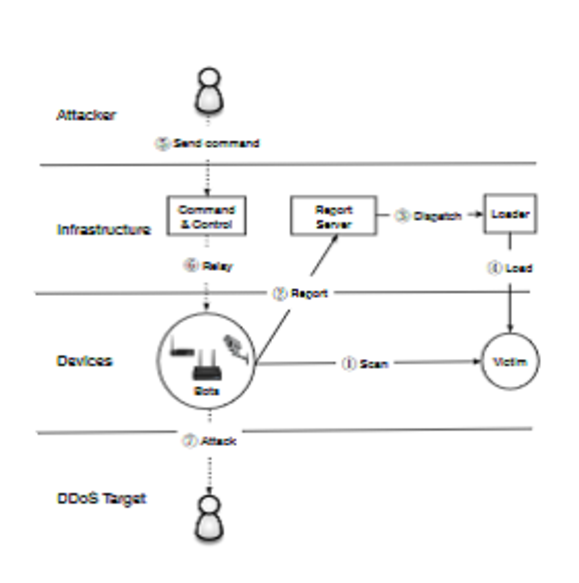
\includegraphics[width=100mm]{figures/s.eps}
      \caption{Miraiの概要図}
   \label{fig:model}
   
\end{figure}

C\&Cサーバーは,ボットやユーザーからの接続されるのを待機しており,主な機能としてボット管理機能,ユーザー管理機能,攻撃指示機能がある.MySQLにはユーザーのリストと攻撃履歴が記録されるようになっている.botは,C\&Cサーバーからのコマンドを待機し,感染先でボットネットに加えられる新しいデバイスを探索するスキャン活動を行う.スキャン活動を行いログインできる端末を見つけた場合には,IPアドレス,ポート,ログイン情報をスキャンサーバーへと送る.感染経路について,Miraiは、Telnetログインが可能な場合に感染する.Loaderは,スキャン活動からレポートサーバーに送られた攻撃対象の情報をもとにTelnetログインを試みる.Telnetログインに成功した際には,攻撃者が用意したhttpサーバーまたはtftpサーバーから,Miraiのバイナリファイルを対象のIoTデバイスにダウンロードしbotを実行させる.botの動作後には,C\&Cサーバーとの通信を始め,C\&Cサーバーから送られてくる攻撃命令を受け取り,IoTデバイスが特定のサーバーに攻撃を始める
.

\section{研究目的}
本研究では,DDoS攻撃を行うマルウェアMiraiとその亜種の未知のマルウェア検知である.

\section{論文の構成}
%書き方がよくわからないので後で確認を行う.
本論文は,1章に背景,2章では関連研究・技術,3,4章では検知手法の提案,5章では評価実験を行い,6章でまとめを述べる. % 序論
\chapter{関連研究・技術}
 
\section{関連研究}

\subsection{DDoS攻撃を行うマルウェアの分析}
DDoS攻撃を行うマルウェアの分析を行った研究が行われている.組込みシステム向けマルウェアMiraiの攻撃性能評価では,MiraiをVM上で動作させ通信の様子や攻撃の流れの動作を確認し,攻撃性能を計測した.ローカルネットワーク上で実機実験として複数の組み込みボード(odroid-c2)を用いてVMと同様にMiraiの動作環境を構築し,攻撃性能の影響の調査を行った.組み込みシステム向けTCP/IPスタックからなるhttpサーバーが動作する静的な組込みシステムのプロトタイプを対象に攻撃を行いDDoS攻撃時には,CPU使用率が大幅に上がることを明らかにした.しかし,研究結果からマルウェアに対して具体的な検知手法の提案がなされていない.
%IoT機器へのTelnetを用いたサイバー攻撃の分析では,
IoTマルウェアによるDDos攻撃の動的解析による観測と分析では,ハニーポットを用いて収集したIoTマルウェアの検体を用いてARM,MIPS,MIPSELの3種類のCPUアーキテクチャを用いてマルウェアを動作させその挙動を観測し,ダミーC\&Cサーバーを用いて攻撃再現実験を行いDoS攻撃の性能について観測を行った.

%\sbusection{動的解析を用いたマルウェア検知の研究}
\subsection{動的解析を行ったマルウェア検知の研究} % subsectionのタイトル

マルウェアの検知手法に関して,APIを特徴として用いた研究が広く行われている.
API呼び出しパターンに着目した検知手法では,API呼び出しパターン,API呼び出しによる経過時間とシステム負荷を特徴量としたマルウェア検知手法を提案した.マルウェア1検体あたりに10間動作をさせ,その間に得られた動的解析ログからAPI呼び出しとそれに伴う経過時間とメモリ使用量の情報を抽出し,マルウェアの特徴抽出を行い,機械学習アルゴリズムを用いてマルウェア検知を行う.結果として,API遷移がほとんど重複していないマルウェアに関しては高い精度で検知を行う事ができた.しかし,呼び出されるAPIがある程度重複しているマルウェア検体を用いた実験を行っていないため,呼び出されるAPIが重複している場合は,検知精度がどの様になるのか明らかにされていない.
実行ごとの挙動の差異に基づくマルウェア検知手法
マルウェアを複数回実行した際の挙動の差異を判断することによってマルウェアの検知を行う.検査対象である1つのマルウェアを2回動的解析を行い,それぞれの実行時のAPI呼び出しログを取得しログから特定のAPIの引数を抽出し2つの実行ログから取得した引数が異なっている場合にマルウェアと判断を行った.しかし,毎回決まった動作を行うマルウェアは挙動の変動が見られないため検知ができなかった.しかしそのようなマルウェアに対してはパターンマッチング方による検知が有効だと考えられ,提案手法と組み合わせた効率的な検知手法の提案が課題になっている.この検知手法では,特定のサーバーにマルウェアだと思わしきバイナリファイルを送信し実行してログを取得しているため,Miraiのように実行後に自身のバイナリファイルを消してしまうマルウェアには有効ではない.
アノマリ手法を用いたIoT機器マルウェア感染検出では,IoTデバイスをもしたハニーポットを用いて多くのマルウェアからダウンロードされたバインリファイル,スクリプトファイルの収集を行った.収集したファイルを用いて動的解析を行い実際に,マルウェアが行う通信を記録した.マルウェアがおこなう通信がIoTデバイスの本来の通信とは異なることを明らかにし,C\&Cサーバーとの通信を検知することによってマルウェアの検知を行った.しかし,C\&Cサーバーとの通信が遮断されていたり,通信が暗号化されている場合には検知ができない.通信以外の挙動を併せて検知することでこの問題は解決可能だと考えられ,マルウェアの多様な挙動が観察可能という点でIoTデバイスでのマルウェアの検知は妥当だと考えられる.

\section{関連技術}

\subsection{Arbor Networks Peakflow}
トラフィック管理技術のNetFlowなどを使用してネットワーク全体をモニタリングし,DDoS攻撃の恐れがあるトラフィックを検知する.疑わしいトラフィックにてついては,DDoS攻撃をさ緩和せるTMSと呼ばれるに中継させ世紀のトラフィックだけを通信させる.このシステムではDDoS攻撃だと思われるトラフィックを検知してから30秒以内にDDoS攻撃の緩和動作を始める.本研究では,30秒以内に検知を行うことを1つの基準として定める.
\subsection{Clam AntiVirus}
Clam AntiVirusはオープンソースで提供されているクロスプラットフォームのアンチウィルスソフトウェアである.シグネチャと呼ばれるマルウェアの特徴を記載したファイルによるパターンマッチング方式を 
採用しており,約21755種類のウィルスに対応をしている.公開されているシグネチャを用いてホスト上にあるファイルをスキャンしシグネチャと一致したファイルが無いか探索を行う.シグネチャと一致するファイルが有った場合には,通知を行う.
 % 関連研究
%\chapter{提案手法}
\chapter{シンボルテーブルを用いた検知手法の提案}

\section{検知手法へのアプローチ}
検知手法を定めるために,IoTデバイス上で普段の動作とマルウェアがダウンロードされ実行されたあとの動作の違いを明らかにする.その後,Miraiを実際に動作をさせデバイス上で行われている動作の解析を行う.実行コマンド,プロセスの2つのログデータの収集を行い,マルウェアが実行される前と後の相違点を明らかにする.

\section{Miraiソースコードを用いた稼働調査}
Miraiの挙動の稼働調査としてWeb上で公開されているMiraiのソースコード\cite{code}を用いてマルウェアが感染する際の感染動作とC\&Cサーバーとの通信が行われ,攻撃命令を待機するまでのマルウェアの動作を確認した.MiraiがIoTデバイスに感染する様子を確認するために,VMを用いた解析環境を図2に示す.Miraiをダウンロードさせ実行させるための感染端末,Loader,C\&Cサーバー,MySQLの4つを用意した.MySQLにC\&Cサーバーの管理ユーザを登録しC\&Cサーバーとbotの通信状態を確認できるようにした.Loaderが感染端末にTelnetログインを行い,感染端末の通信が確立される.ログイン後に実行されるコマンドの収集を行い、表1に示すコマンド列を得た.
\begin{table}[t]
   \caption{表1 マルウェアによる実行コマンド}
   \centering
\begin{tabular}{p{7cm}}
\hline
/bin/busybox wget;\\
/bin/busybox wget http://192.168.32.10:80/bins/mirai.x86 -O -\textgreater dvrHelper;\\
/bin/busybox chmod 777 dvrHelper;\\
./dvrHelper telnet.x86;\\
\hline
\end{tabular}
\end{table}表1のようにMiraiはバイナリファイルをダウンロードした際に,バイナリファイルの名称をdvrHelperに変更している・しかし,バイナリファイルの実行後に,psコマンドでプロセス名を確認すると,無作為なプロセス名で動作し,他の端末からTelnetログインができなくなっていることが確認された.Miraiには,DDoS攻撃を行う機能だけではなく,特定のポートを閉じる機能やプロセス名を無作為にする機能が存在することが確認された.
 \begin{figure}[h]
 \centering
    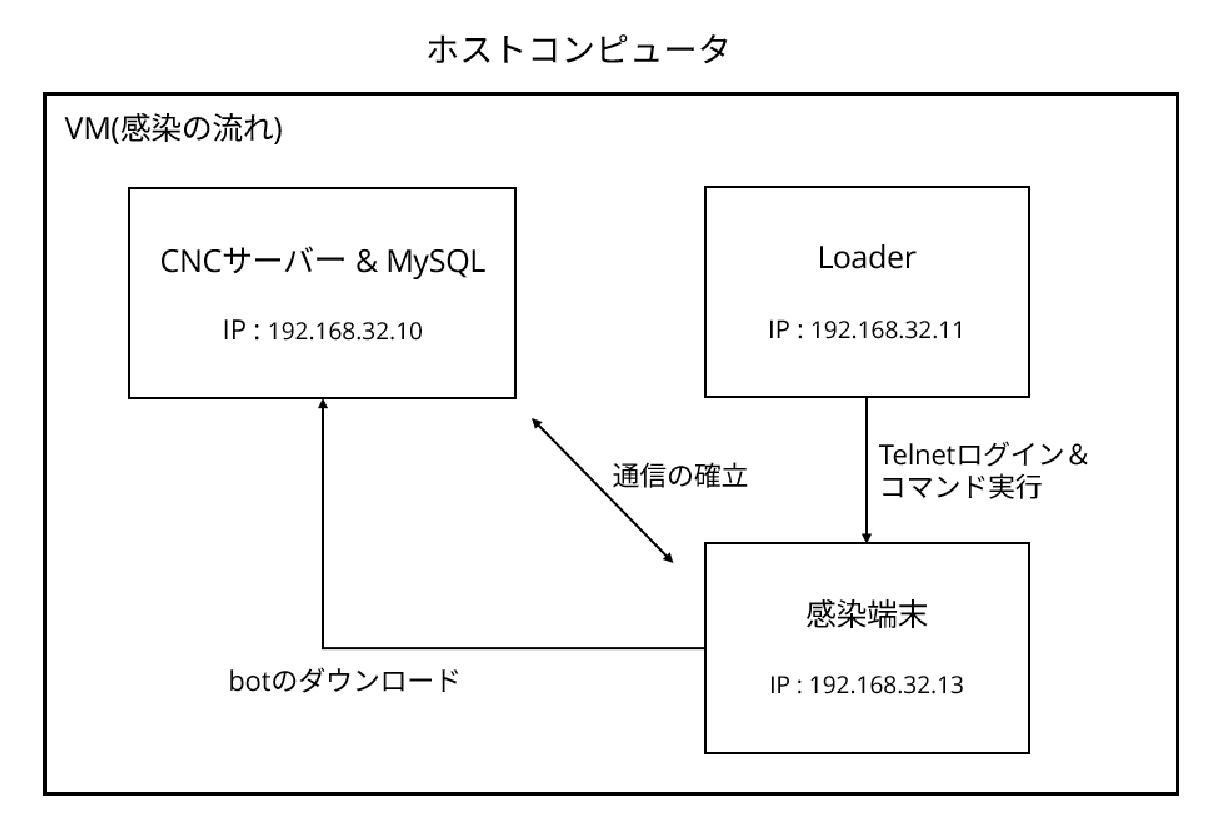
\includegraphics[width=100mm]{figures/VM.eps}
    \caption{Miraiの解析環境}
 \label{fig:model}
 \end{figure}
 \newpage

\section{シンボルテーブルを用いた検知手法の提案}
計算資源が潤沢でないIoTデバイス上でも実現可能な,Mirai亜種の動作を検知する軽量な動的解析に基づく検知システムを提案する.検知システムの概要を図3に示す.Miraiとその亜種であるOwariを含めて調査したところ,DDoS攻撃を行うマルウェアについて亜種を含めて同様の機能を持つ,同一のコードが再利用されていることが確認された.そこで,マルウェアが持つ特定の関数の具備を検知条件として定め,この条件を満たすプロセスの稼働を検出することによってマルウェア感染の有無を判定する手法を以下に述べる.

\begin{enumerate}
 \item IoTデバイス上で動作を行うプロセスのホワイトリストを作成する.ホワイトリストとは,端末上で可動が許可されたプロセスリストのことである.
 \item プロセスを監視し、作成されたホワイトリストをもとに記載がないプロセスを発見する.
 \item ホワイトリストにないプロセスに関して,プロセスを動かしているバイナリファイルのシンボルテーブルを確認し,プロセス名を無作為に変更するなどのマルウェアの特定の関数が存在しているか確認を行う.
 \item マルウェアが持つ特定の関数の存在が確認できた場合には,マルウェアだと判断を行う.
 \item ホワイトリストにないプロセスに関して,シンボルテーブルの探索が終わった場合には2に戻る
 \end{enumerate}

 検知項目でマルウェアが持つ特定の関数として,DDoS攻撃を行う関数や,事前調査で把握した,プロセス名を無作為にする関数や,特定のポートを閉じる関数などが候補に挙げられる.
 
 \begin{figure}[h]
 \centering
    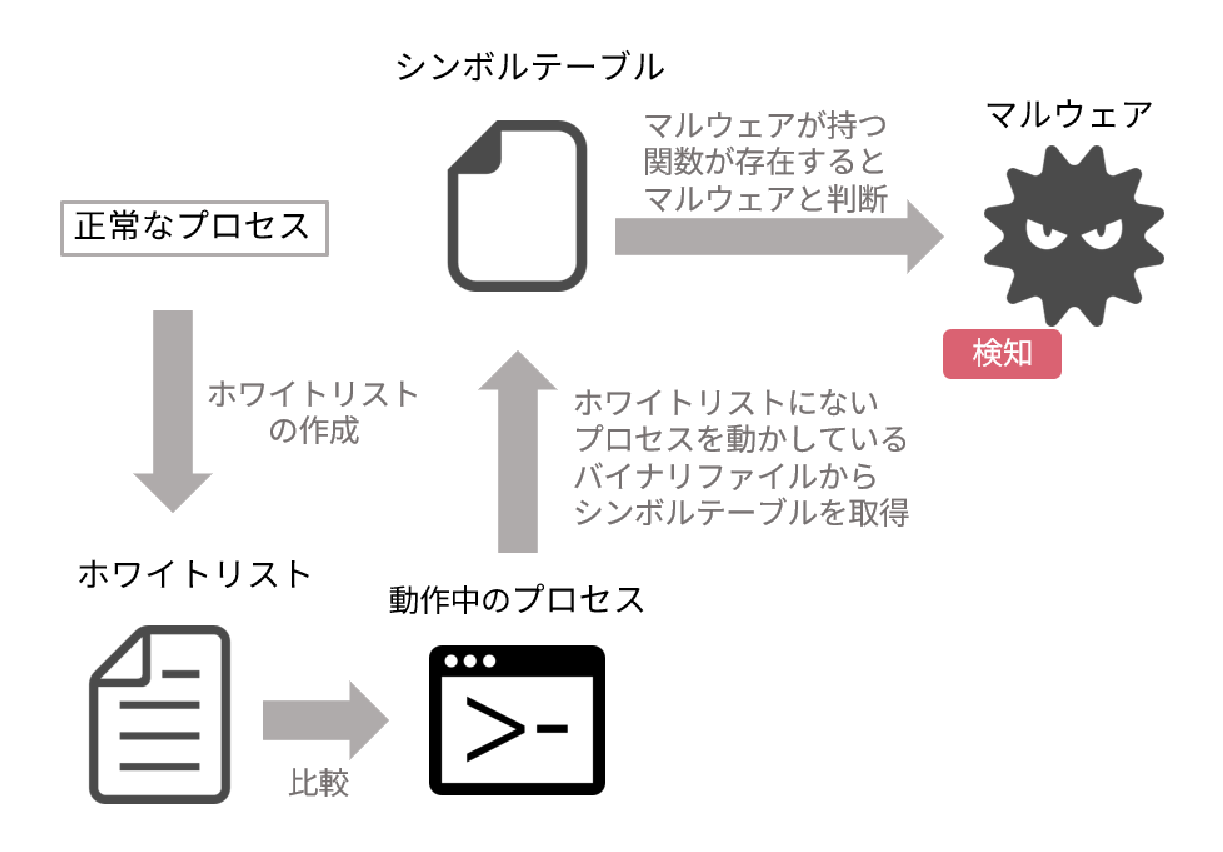
\includegraphics[width=120mm]{figures/system.eps}
    \caption{検知システムの概要}
    \label{fig:model}
 \end{figure}
 
\newpage


%掲載したグラフから何を読み取るべきかきちんと数値で言及をする.
\section{マルウェア探索動作による負荷と検知における制約事項}
IoTデバイスは放置されることが多く,常に操作を行っているわけではない.そのため継続的にアンチウィルスソフトウェアなどの検知システムを利用してIoTデバイスにマルウェアがダウンロードされ実行されていないか確認をし,IoTデバイスが安全な状態であることを把握する必要がある。検知システムのマルウェア探索動作によって,IoTデバイスの動作が妨げられる可能性がある.検知システムの動作を行っている際のIoTデバイスの状態はマルウェアが動作している状態とマルウェアが動作していない2種類に分類される.IoTデバイス上でMiraiなどDDoS攻撃をおこなうマルウェアが動作している際には,特定のサーバーに対してDDoS攻撃を行ってしまうためIoTデバイスの正常な動作を妨げてまでマルウェアを検知する必要がある.しかし,IoTデバイス上でマルウェアが動作していない状況下において映像,音声,ログなどの様々なデータを伝達するため動作等がマルウェアの探索動作によって阻害されてはならない.そのため,IoTデバイスにマルウェアが動作していない状況下において,提案した検知システムによるマルウェア探索動作がIoTデバイス本来の動作を阻害していないか評価を行う.また,IoTデバイスにMiraiが動作した場合に,提案した検知システムによって検知が可能であることを評価する.提案手法の可動に必要なマルウェア探索動作によってIoTデバイス本来の動作が阻害されてないことを評価するために,LinuxOSを対象とする既存のアンチウィルスソフトであるClam AntiVirusを動作させた状態のCPUとメモリ使用率をそれぞれ基準値とし,提案手法によるマルウェア探索動作の動作負荷について比較を行い,併せて提案手法によってMiraiマルウェアの検知が可能であることを確認した.提案した検知システムによってMiraiが動作していない状況での、CPU,メモリの使用率についてsarと呼ばれるシステムの負荷状況を確認するコマンドを用いて1分間計測を行なった.表のスペックのラズベリーパイを利用し負荷状況を測定した.
\begin{table}[h]
   \caption{評価環境のIoTデバイスのスペック}
   \centering
   \begin{tabular}{|l|c|l|l|l|}
   \hline
   \multicolumn{1}{|c|}{評価環境のIoTデバイスのスペック}                                  \\ \hline
   OS     & \multicolumn{2}{c|}{Openwrt 4.9.120}                   \\ \hline
   CPU    & \multicolumn{2}{c|}{Quad Core 1.2GHz Broadcom BCM2837} \\ \hline
   MEM    & \multicolumn{2}{c|}{1GB}                               \\ \hline
   \end{tabular}
   \end{table}

%!!!!!!!!!!!!!!!!!!!!!!!!!!!!!!!!!!!!!!!!!!!!!!!!!!!!!!!!!!!!!!!!!!!!!!!!!!!!!!!!!!!!!!!
%!評価に用いた評価環境を記載する(まだ記載されていない).対象のIoTデバイスのスペック等々!
%!!!!!!!!!!!!!!!!!!!!!!!!!!!!!!!!!!!!!!!!!!!!!!!!!!!!!!!!!!!!!!!!!!!!!!!!!!!!!!!!!!!!!!!

sarコマンドを用いて得たCPU,メモリの使用率についてClam AntiVirusと提案した検知システムの比較を行った結果が図4,5になる.Clam AntiVirusを利用した場合には,平均CPU使用率が25.28\%,メモリ使用率は7.93\%となった.提案した検知手法では,平均CPU使用率が3.03\%,メモリ使用率が7.21\%となった.メモリ使用率は比較対象のClam AntiVirusと提案した検知手法では12.5\%減,CPU使用率は,Clam AntiVirusに対して提案した検知手法は88\%減となったことからマルウェアの可動を検知する目的で一般的によく利用されるClam AntiVirusに比較して提案手法の実装では資源消費が少なく他のプロセスの動作を妨げる可能性は低いと言える.しかし,提案した検知した検知手法は実行形式ファイルに含まれるシンボルテーブルの内容に基づいている為,マルウェアの実行形式ファイルに対してstripコマンドを用いるなどしてシンボルテーブルが削除された場合には検知が行えないという課題がある.

\begin{figure}[h]
 \centering
    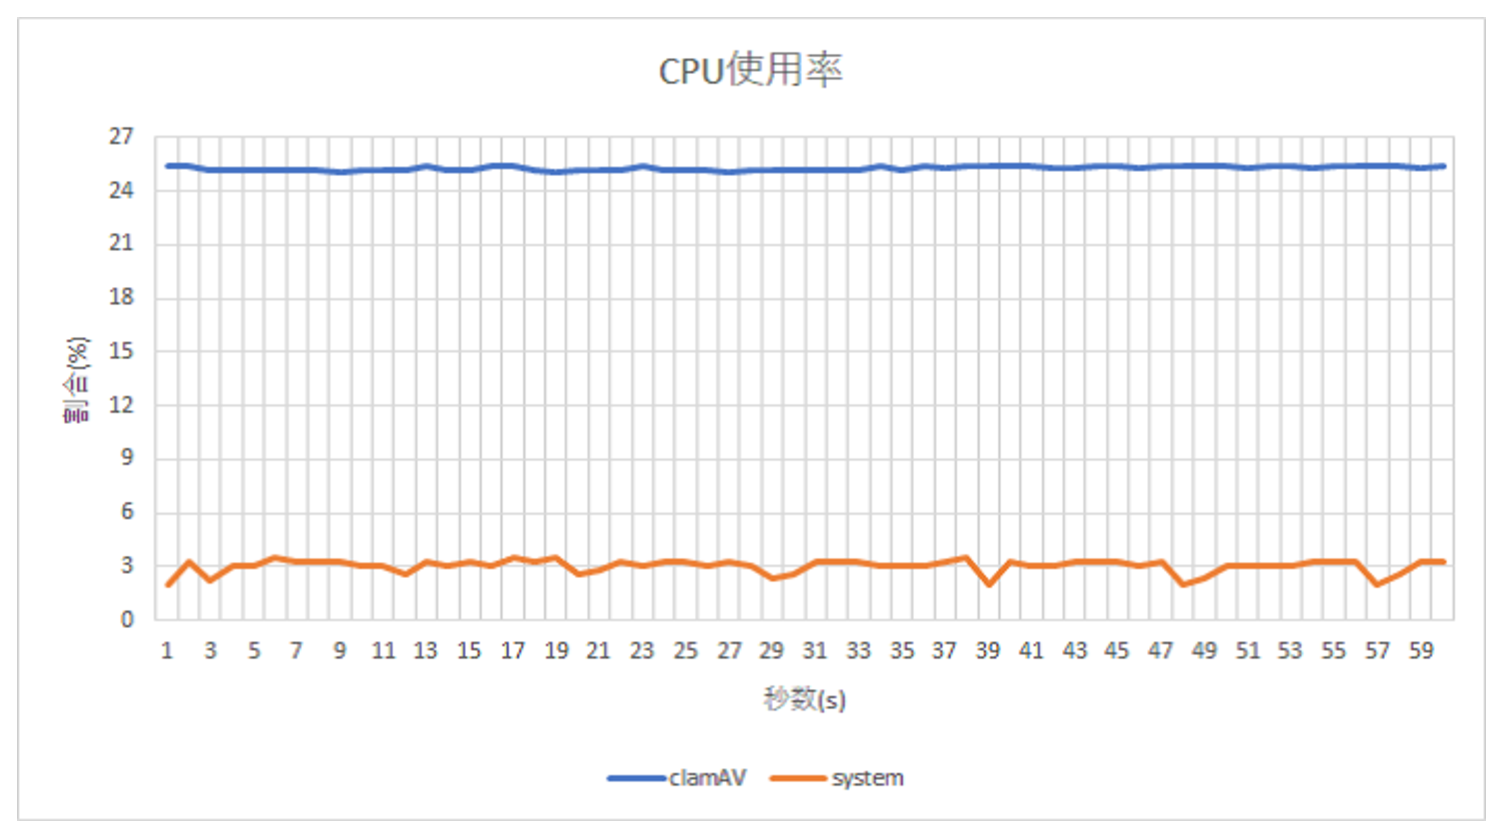
\includegraphics[width=120mm]{figures/CPU.eps}
 \label{fig:model}
 \caption{IoTデバイス上でマルウェアが動作していない状況下におけるマルウェア探索のメモリ使用率}
 \end{figure}
 
 
\begin{figure}[h]
 \centering
    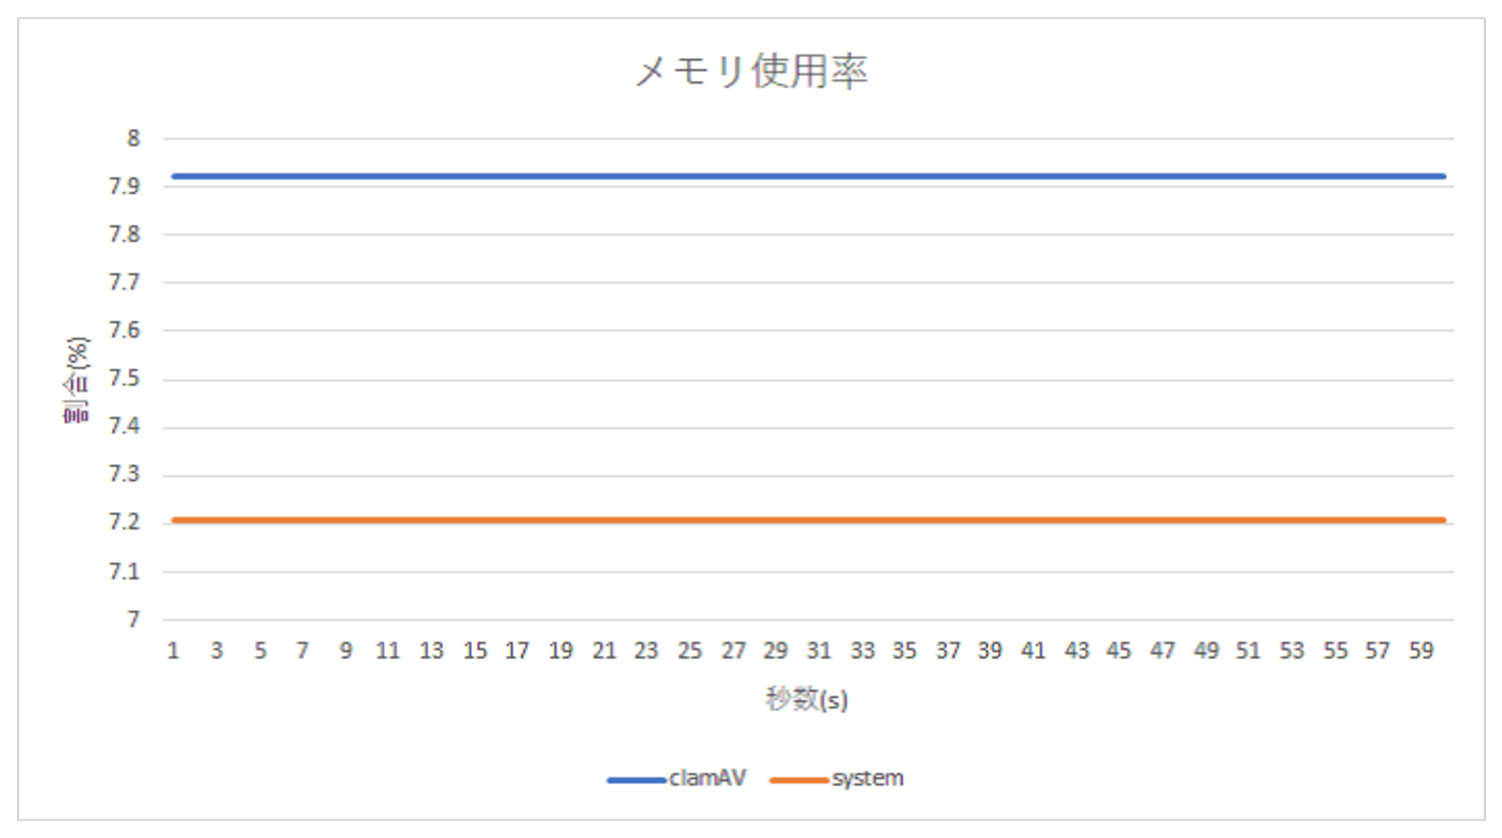
\includegraphics[width=120mm]{figures/mem.eps}

   \caption{IoTデバイス上でマルウェアが動作していない状況におけるマルウェア探索のCPU使用率}
    \label{fig:model}
 \end{figure}
 % 検知手法・提案手法
\chapter{システムコール呼び出し履歴を用いた検知手法の提案}

\section{新たな検知手法の必要性}
前章で述べたシンボルテーブルを用いてマルウェアの検知を行う検知手法では,stripコマンドを用いてシンボルテーブルを削除したり,検知条件となっている関数名を変更するといった攻撃者側による検知回避の対処が取られた際には有効な検知が行えないという課題がある.しかし,関数が呼び出すシステムコールの呼び出し順番は関数名の名称を変更しただけでは変化しない.straceと呼ばれる動作しているプロセスから呼び出されているシステムコールを追跡するコマンドを用いて,Miraiマルウェアのプログラムにおいて特徴的な動作を実装した内部関数に着目しこの関数から呼び出されるシステムコールの系列を用いた検知を行うことによって検知回避の対処がなされた場合でも検知が可能になる.


%書くべきこと
%スキャン動作に着目した理由

\section{Miraiの特徴的な動作に基づく検知条件知手法}
Miraiマルウェアは特徴的な動作として,サーバーにDDoS攻撃を行う動作の他にインターネットに公開されているホストに対して新たな侵入先を見つけるためにtelnetログインが可能な端末をスキャンする活動を行っている.また,MiraiはサーバにDDoS攻撃を行うプロセスとtelnetログインが可能な端末をスキャンする活動のプロセスは独立して動作しているため,プロセスは別々に存在している.DDoS攻撃を行うプロセスはDoS攻撃を行っている場合や,攻撃命令を待機している挙動など動的解析を行うタイミングによって,異なった解析結果が得られることが考えられる.しかし,スキャン活動を行うプロセスはログインできる端末を探索している挙動が主なため動的解析を任意のタイミングで行っても,共通している解析結果が得られると考えられる.DDoS攻撃を行うためのプロセスとスキャン活動を行っているプロセスについてstraceを用いてシステムコールを追跡したところ,DoS攻撃を行うプロセスは攻撃命令を待機している状態になるまでに呼び出されるシステムコールは様々なものがあった.しかし,スキャン活動を行っているプロセスはsendtoと呼ばれるソケットへメッセージを送るシステムコールを連続して呼び出していた.そのため,任意のタイミングでstraceをおこないシステムコールを追跡しても同様の結果を得ることができる.なので,スキャン活動を行うプロセスに着目をしスキャン活動が呼び出すシステムコールの系列を用いた検知を行う.スキャン活動を行うプロセスのシステムコールの実行状況を追跡したところsendtoを連続して呼び出しており,sendtoによって送信されるメッセージの宛先アドレスが呼び出しごとに異なったアドレスであること,送信先のポートが23であったことからこのシステムコールを検知に用いる特徴とする.検知条件として3つの条件を定める.

\begin{enumerate}
\item sendtoのシステムコールが2回以上連続して呼び出されていること
\item sendtoによって送信先のポートが23であること
\item sendtoによって送信されるメッセージの宛先アドレスが呼び出しごとに異なったアドレスであること
\end{enumerate}


\section{誤検知の可能性}
前章で述べた検知条件をもとにマルウェア探索を行った際に,誤検知する場合として,以下の3つが考えられる

\begin{enumerate}
\item IoTデバイス上でsendtoの呼び出しが多いプログラムの実行
\item IoTデバイスから複数の端末に向けてメッセージを送信
\item IoTデバイスから複数の端末を遠隔操作しサーバー等の設定やログファイルを特定のサーバーへ転送
\end{enumerate}

straceを用いてシステムコールを確認し上記の動作が検知条件に一致するのか確認を行った.IoTデバイス上でsendtoの呼び出しが多いプログラムが実行されるプログラムとして,一定時間sendtoのみを呼び出すプログラムについて考える.sendtoが呼び出されるだけのプログラムでは,検知条件に一致しやすく誤検知する可能性がある.しかし,送信先のポートが23であり,送信されるメッセージの宛先がすべて別の宛先アドレスであるsendtoが呼び続ける正規プログラムが存在するとは考えにくい.IoTデバイスから複数の端末に向けてメッセージを送る動作として考えられるものが,wallやwriteなどIoTデバイスにtelnet,sshログインしている端末にメッセージを送るコマンドがある.wall,writeコマンドを実行してシステムコールを確認した結果が表2のようになる.%システムコールの結果を入れる
表2のようにsendtoを呼び出すことが確認されなかったため,IoTデバイスから複数の端末に向けてメッセージを送信する場合には誤検知することがない.IoTデバイスから複数の端末を遠隔操作する方法について,sshやtelnet,parallel-sshといったリモートシェルを用いて手動でコマンドを入力して端末を操作する場合とスクリプトファイルなどで端末を自動的に操作させる2種類がある.IoTデバイスから複数端末を手動でコマンドを入力してファイルの転送などを行いシステムコールを確認した結果,sendtoを連続では呼び出していなかった.スクリプトファイルを利用してファイルの転送を行う場合も,同様にsendtoを連続で呼び出していることを確認できなかった.sendtoだけを呼び出すプログラムをtelnet,sshを使用して端末上で実行した場合,本来はシステムコールであるsendtoが連続で呼び出されていたものがsendtoの次にwirteのシステムコールが呼び出されsendtoが2回以上連続で呼び出されていることが確認できなかった.sshやtelnetを利用して遠隔操作を行う場合や他の端末にメッセージを送信する場合にはsendtoが2回以上連続で呼び出されていることがないため誤検知することはないと考えられるため,これらの検知条件は妥当だと考える.

%実験環境も記載する
\section{straceコマンドによる監視対象のプロセスの実行速度の調査}

%あとで編集を行うようにする.
straceコマンドによってシステムコール呼び出し履歴を監視されるプロセスの実行速度が低下することが考えられる.そのため,straceコマンドによってプログラムの実行速度の変化を調べstraceによるシステムコールの監視動作がプロセスに与える実行速度の影響を調査した.使用するプログラムとしては,農林水産研究情報総合センターが定める,よく使用されるLinuxコマンド\cite{Linux}を使用した.cp,tar,df,ps,catの5つのコマンドを対象にstraceによるシステムコールの監視動作によるプロセスの実行速度の影響を調査した.実行したコマンドはは表\ref{tab:command}になる.
\begin{table}[h]
   \caption{実行したコマンド}
   \label{tab:command}
   \centering
    \begin{tabular}{clll}
     \hline
     \hline
     cat gpl-2.0.txt \\
     cp gpl-2.0.txt cp.txt \\
     ps -w \\
     df \\
     tar -zcvf gpl-2.0.tar.gz gpl-2.0.txt \\
     \hline
    \end{tabular}
\end{table}

  コマンドの引数にファイルが必要になる場合にはフリーソフトライセンスであるGPL2の内容が書かれているテキストファイルを使用した.表\ref{tab:command}%表を入れる
  の5つコマンドに対してのstraceコマンドを実行した場合の速度比較を行った.実行した結果が表\ref{tab:strace_result}になる.

\begin{table}[h]
   \caption{計測結果} 
   \label{tab:strace_result}
   \centering
  \begin{tabular}{|l|l|l|}
   \hline
   \multicolumn{1}{|c|}{} & 無為(秒)   & strace(秒) \\ \hline
   cat                    & 3.5730  & 3.6894    \\ \hline
   cp                     & 0.0048  & 0.2517    \\ \hline
   ps                     & 0.5134  & 10.9312   \\ \hline
   df                     & 0.6264  & 0.1212    \\ \hline
   tar                    & 0.57014 & 0.0294    \\ \hline
   \end{tabular}
\end{table}

システムコールの監視動作による速度はcatコマンドは3\%低下,cpコマンドは5079\%低下,psコマンドは2029\%低下,dfコマンドは417\%低下,tarコマンドは1839\%低下.この結果から,呼び出されるシステムコールによって速度の低下量は変化するがシステムコール監視動作によってプロセスの実行速度は低下することがわかった.システムコール監視対象となるプロセスが正常なプロセスだった場合,実行速度の低下がするため,マルウェア探索動作による1プロセスあたりのstraceの実行回数,アタッチする時間を短くする必要がある.


%行うことリスト
%\begin{enumerate}
%   \item よく実行されるコマンドのプロセスについて調べる
%   \item よく実行されるコマンドについてstraceをおこない実行する際のstraceのオーバーヘッドの量を調べる
%   \item コマンドに存在するシステムコールについてstraceを行い,straceのオーバーヘッドの量を調べる
%   \item 結果からstraceを使用することによってプロセスの実行時間が伸びるために提案システムでstraceを行う回数をへらすことを反す
%\end{enumerate}

%システムの概要図は挿入されているか
\section{システムコール呼び出し履歴を用いた検知手法の提案}
計算資源が潤沢でないIoTデバイス上でも実現可能な,Mirai亜種の動作を検知する軽量な動的解析に基づく検知システムを提案する.検知システムの概要を図\ref{fig:strace}に示す.Miraiはtelnetログインが可能な端末を探索するスキャン活動を行う機能を持ち,システムコールの一種であるsendtoを複数回連続で呼び出している.そこで動作しているプロセスからシステムコール呼び出し履歴を取得し,スキャン活動を行っているプロセスの動作を確認することでマルウェア感染の有無を判定する手法を以下に述べる.

\begin{enumerate}
 \item IoTデバイス上で動作を行うプロセスのホワイトリストを作成する.
 \item プロセスを監視し、作成されたホワイトリストをもとに記載がないプロセスを特定する.
 \item 特定した複数のプロセスに関して,straceを1秒間実行し検知条件に一致したシステムコール呼び出し呼び出し履歴があるか監視する.もし検知条件に一致したシステムコール呼び出し履歴があった場合にはマルウェアだと判断を行い通知を行う.
 
 \item 1プロセスあたりのstraceによるシステムコール監視動作の回数を減らすために,
 straceを実行したあとに監視動を中断する時間を設ける.マルウェアを検出するのに要する時間の最悪値を30秒とし,監視動作を中断する時間は以下の式で求める.
 \begin{eqnarray}
 中断時間  =  \frac{最悪値}{監視プロセス数}-1
 \end{eqnarray}
 \item 複数の監視対象となるプロセスに対してstraceを実行する.すべての監視対象となるプロセスに対してstraceを実行した場合には2に戻り繰り返す.
 \end{enumerate}
 
 検知システムとして前章で述べたシンボルテーブルを用いた検知システムに変更したものを利用した.

 %%%%%%%%%%%%%%%%%%%%%%%%%%%%%%%%%%%%%%%%%%%%%%%%%%%%%%%%%%%%%%%%%%%%%%
 % マルウェアの探索動作についてstraceをする回数を少なくしてもいい理由を書く
 % straceをするタイミングで検知できるかどうか変わらないのか変わらないならその理由を書く              
%%%%%%%%%%%%%%%%%%%%%%%%%%%%%%%%%%%%%%%%%%%%%%%%%%%%%%%%%%%%%%%%%%%%%%%

 \begin{figure}[h]
 \centering
    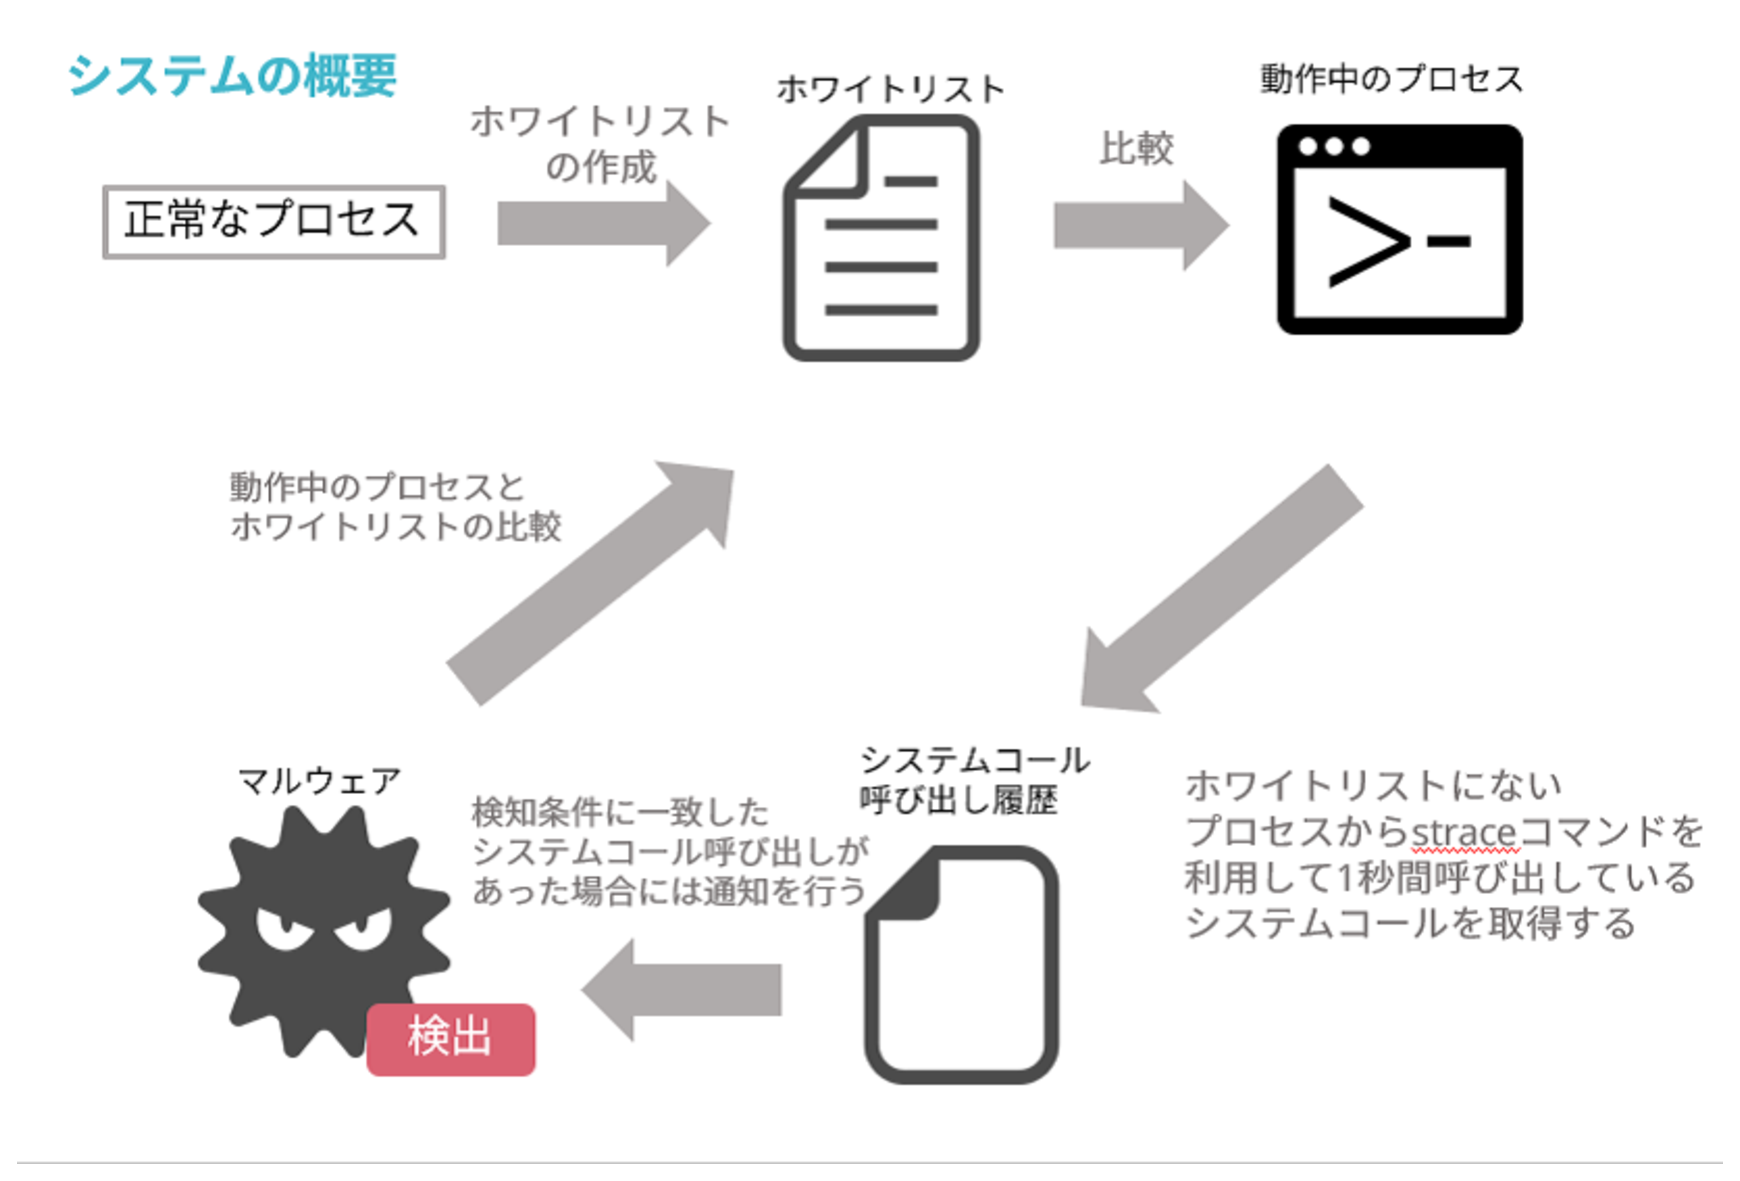
\includegraphics[width=100mm]{figures/strace.eps}
\caption{システムコール呼び出し履歴を用いた検知システムの概要}
\label{fig:strace}
 \end{figure}
 

 % 検知手法・提案手法
\chapter{システムコール呼び出し履歴を用いた検知手法による評価実験}
本研究で実装した検知システムにおける定常的な動作負荷の計測を行い,IoTデバイスが本来の動作を阻害しないことを評価する.DDoS攻撃を行うマルウェアを用いて検知精度の評価を行い,システムコール呼び出し履歴による検知手法でマルウェアが検出できることを確認した.

\section{システムコール呼び出し履歴を用いた検知手法による定常的な動作負荷の評価}

IoTデバイスにマルウェアが動作していない状況下において,提案した検知システムによるマルウェア探索動作によってIoTデバイス本来の動作が阻害されていないことを評価するために,3.4節で述べたように,LinuxOSを対象とする既存のアンチウィルスソフトであるClam AVを動作させた状態のCPU,メモリの使用率を基準値とし,提案した検知システムによってMiraiが動作していない状況での,CPU,メモリの使用率についてsarコマンドを用いて1分間計測を行った.
sarコマンドを用いて得たCPU,メモリの使用率について,Clam AVと比較を行った結果が図\ref{fig:strace_cpu},\ref{fig:strace_mem}になる.ClamAVを動作させた状態のIoTデバイスのCPU使用率,メモリ使用率の値は3.4節で計測したデータを用いた.
Clam AntiVirusを利用した場合には,平均CPU使用率が24.27\%,メモリ使用率は7.92\%であり.提案した検知手法では,平均CPU使用率が0.57\%,メモリ使用率が4.08\%となった.CPU使用率は比較対象のClam AntiVirusと提案した検知手法では97.6\%減,メモリ使用率はClam AntiVirusに対して提案した検知手法は48.4\%減となった.


\clearpage
\begin{figure}[h]
    \centering
       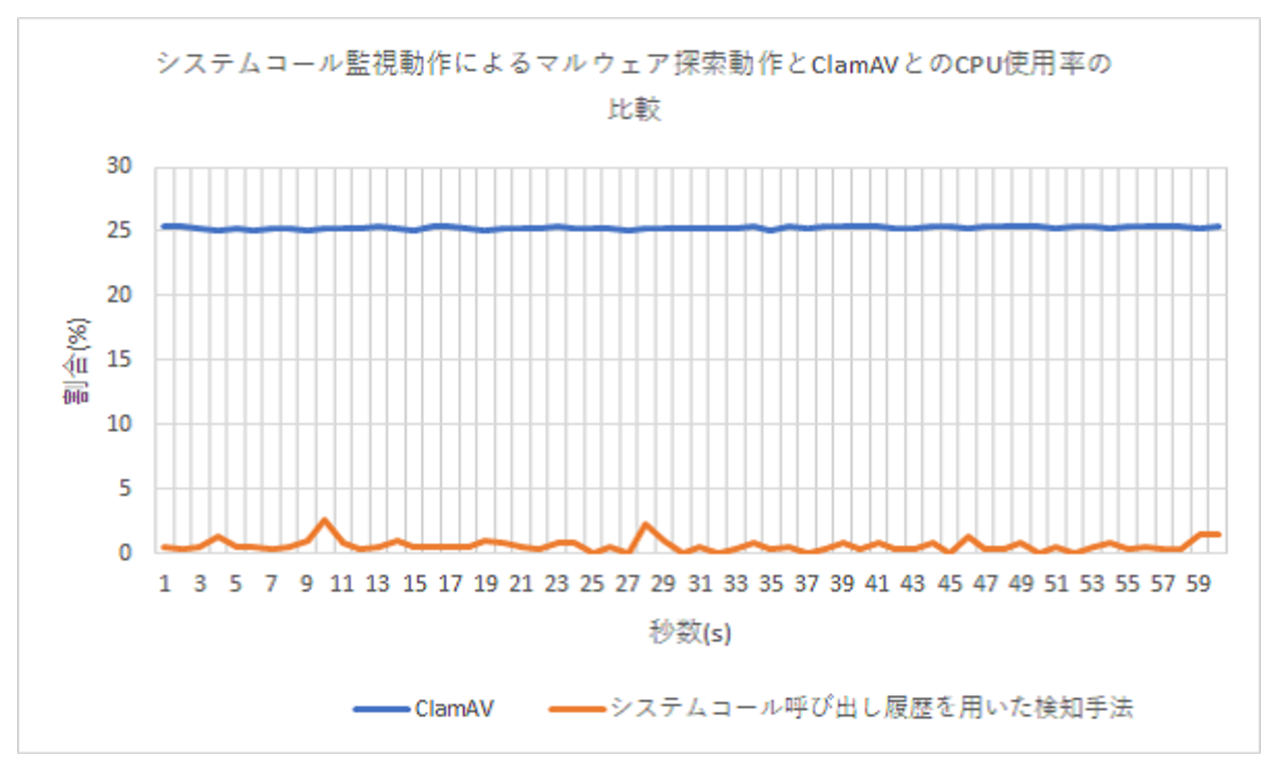
\includegraphics[width=110mm]{figures/strace_cpu.eps}
    \caption{システムコール呼び出し履歴によるマルウェア探索動作とClamAVとのCPU使用率の比較}
        \label{fig:strace_cpu}
\end{figure}
  
\begin{figure}[h]
        \centering
           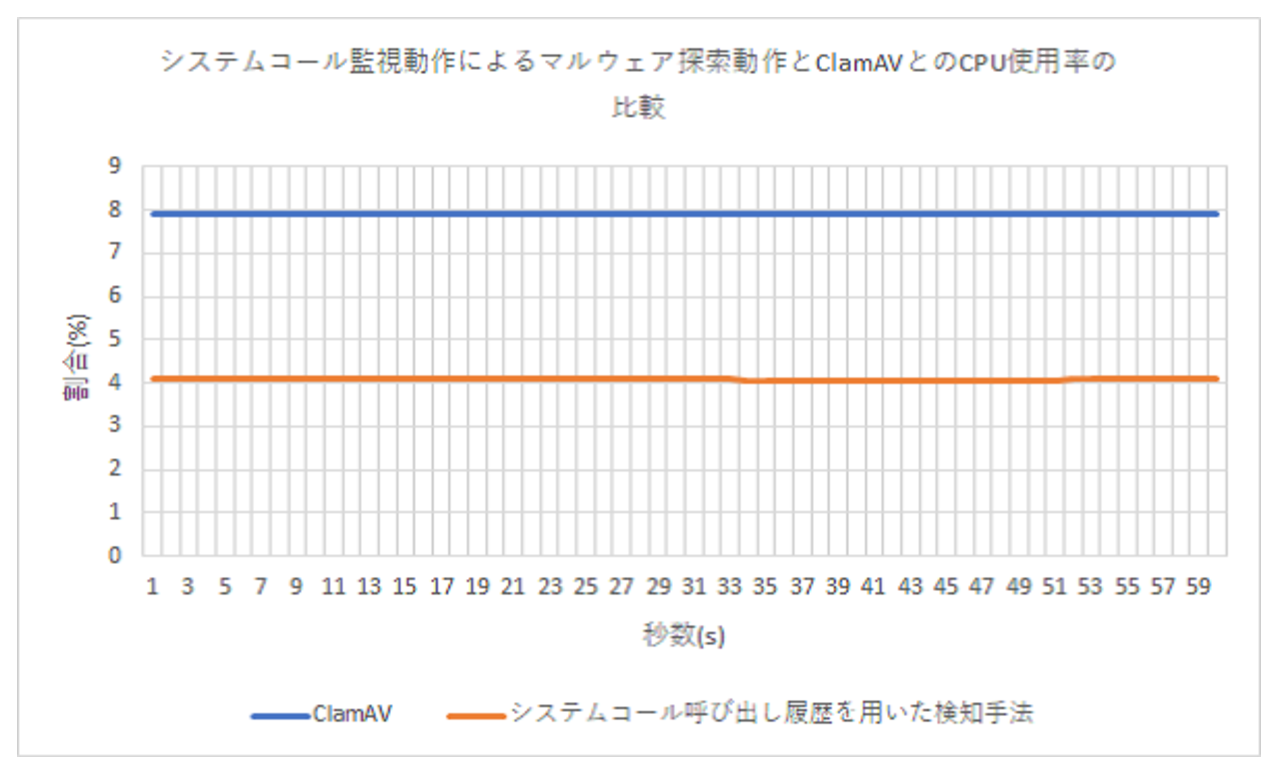
\includegraphics[width=110mm]{figures/strace_mem.eps}
        \caption{IoTデバイス上でマルウェアが動作していない状況におけるマルウェア探索のメモリ使用率}
        \label{fig:strace_mem}
\end{figure}
\newpage
\section{Miraiとその亜種マルウェアを対象とする判別性能評価}
ハニーポットを用いてDDoS攻撃を行うマルウェアを収集し,収集したマルウェアを検体として用いて,システムコール呼び出し履歴を用いた検知手法の検知精度の評価を行い,システムコール呼び出し履歴を用いた検知手法の有効性を確認した.

\subsection{ハニーポットによるマルウェアの収集}
%ハニーポットの説明をもう少し冗長に書いて置く,
ハニーポットと呼ばれる攻撃者に脆弱なシステムであると見せかけることで攻撃者を誘い込み,侵入手法や侵入後に実行されるコマンドのログやダウンロードされるファイルを収集するシステムを用いてDDoS攻撃を行うマルウェアを収集した.ハニーポットのシステムの概要図を図\ref{fig:honey}に示す.シェルの対話の中でダウンロードされるバイナリファイルを実行させることなく保存することが可能なMichel Oosterhofによって開発されたCowrie\cite{Cowrie}と呼ばれるハニーポットを用いた.Cowrieによって収集されたバイナリファイルについてVirus Totalと呼ばれるマルウェア検知オンラインサービスを用いて解析を行い,DDoS攻撃を行うマルウェアの分類を行った.Virus Total\cite{Virus}はユーザーから投稿された検体を54のウィルス対策エンジンによって解析するオンラインサービスであり,投稿された検体についてマルウェアの分類を知ることができる.2019/01/09から2019/01/28の期間でハニーポットを断続的に運用してバイナリファイルの収集を行った.収集したバイナリファイルをVirus Totalに投稿し,Virus Totalの解析結果から,MiraiまたはMiraiの亜種のマルウェアをDDoS攻撃を行うマルウェアとして分類分けした.分析した結果,収集したバイナリファイルは,空ファイルのものや,マルウェアをダウンロードさせ実行させるファイル,DDoS攻撃を行うマルウェアのバイナリファイル等が散見され,DDoS攻撃を行うマルウェアは57検体が存在し,マルウェアの実行可能な検体は49検体であった.評価に用いたマルウェアの検体の情報は付録Aに記載する.
%マルウェアの検体についてそれぞれの名称や種類,検知できたのか,できなかった理由の分類,を表にまとめて記載する.
\begin{figure}[h]
    \centering
       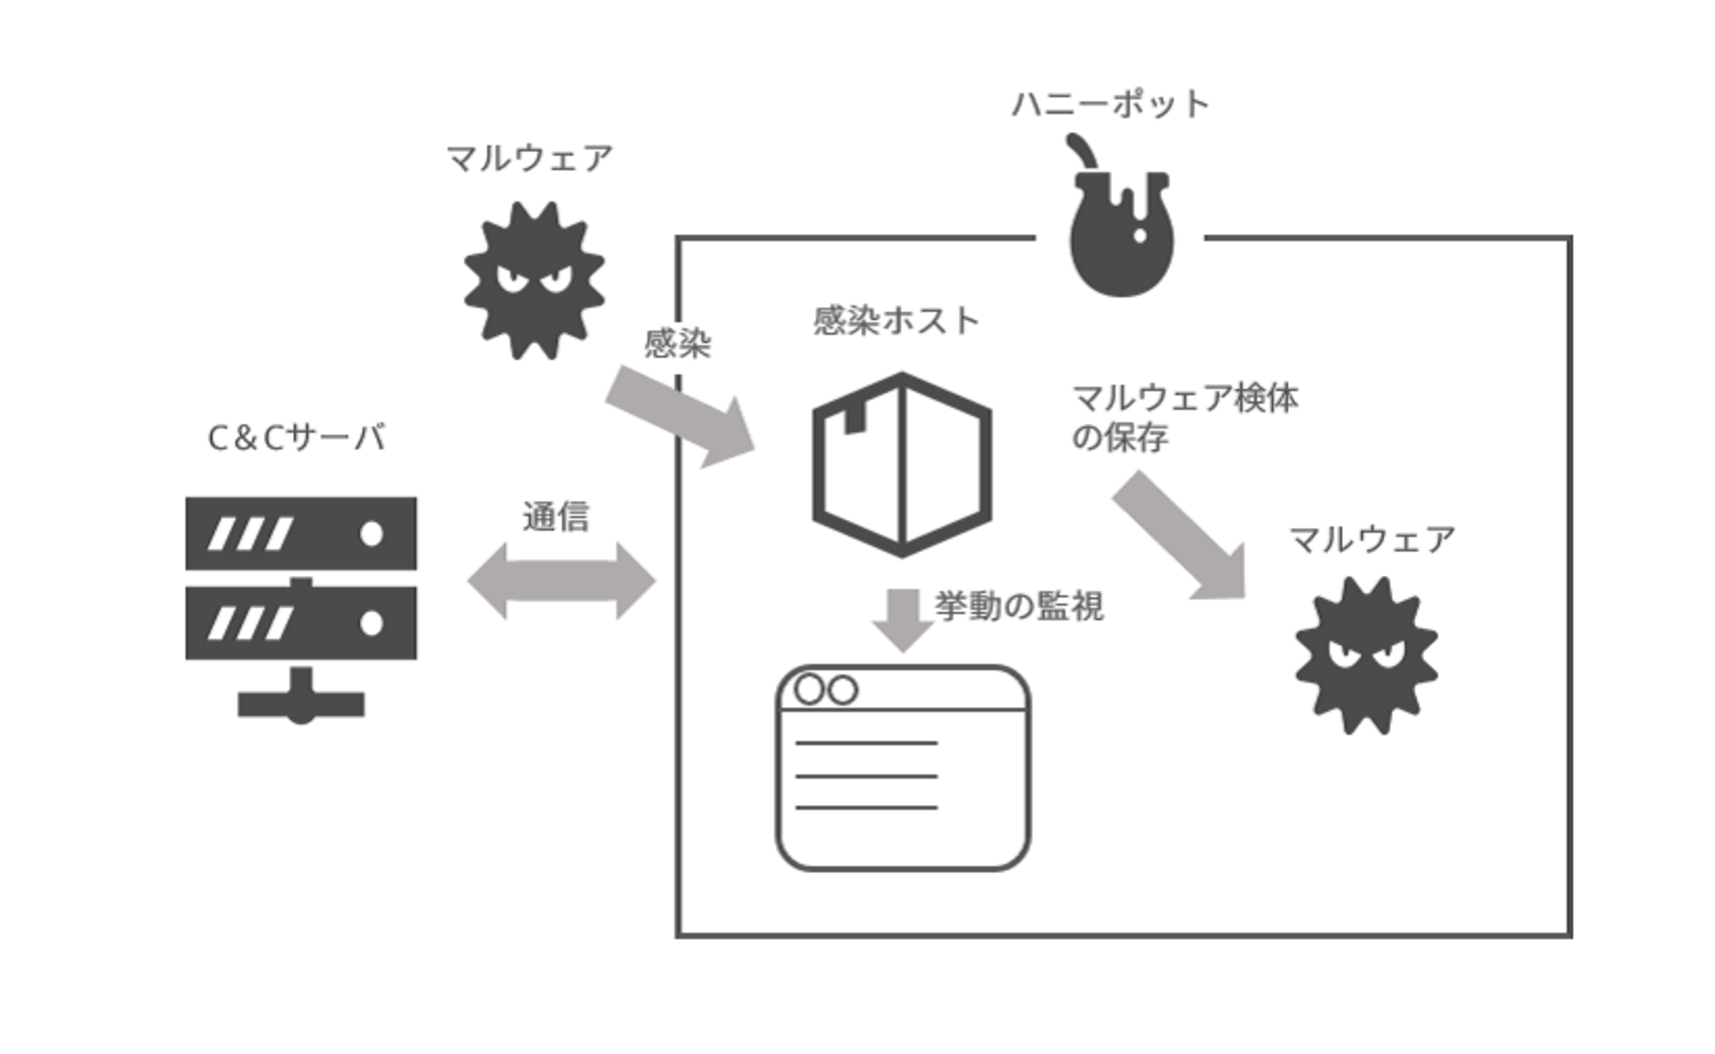
\includegraphics[width=120mm]{figures/honey.eps}
    \caption{ハニーポットのシステム概要図}
    \label{fig:honey}
\end{figure}

\newpage 
\subsection{提案手法によるマルウェアの検知精度評価}
%Linuxのディストリビューションについて明記しておく.
前項で収集したDDoS攻撃を行うマルウェア49検体を用いてシステムコール呼び出し履歴を用いた検知手法の検知精度の評価を行った.入手したマルウェアをネットワークから隔離した状態で検知システムを動作させマルウェアの検出ができるか評価を行った.正規プログラムは,Linuxであるubuntu  16.0 LTS4 LTSに標準でインストールされているプログラムの44検体を利用した.実験の評価指数として,Accuracy,TPR(True Positive Rate),TNR(True Negative Rate),FPR(False Positive Rate),FNR(False Negative Rate)を用いる.Accuracyは,マルウェアを正しく判別できた割合である.TPRはマルウェアをマルウェアと判別できた割合,TNRは正規プログラムを正規プログラムと判別した割合,FNRはマルウェアを正規プログラムと判別した割合,FPRは正規プログラムをマルウェアとして判別した割合である.Accuracy,TPR,TNR,FPR,FNRを下記の式で算出する.

\begin{eqnarray}
    Accuracy & = & \frac{正しくマルウェアと判別された検体数}{検体の総数}\\
    TPR & = & \frac{マルウェア検体がマルウェアと判別された検体数}{マルウェア検体の総数}\\
    TNR & = & \frac{正規プログラムを正規プログラムとして判別された検体数}{正規プログラムの総数}\\
    FNR & = & \frac{マルウェア検体が正規プログラムとして判別された検体数}{マルウェア検体の総数}\\ 
    FPR & = & \frac{正規プログラムをマルウェアとして判別された検体数}{正規プログラムの総数}
\end{eqnarray}
提案システムによるハニーポットで収集したマルウェアの判別結果を表\ref{tab:malware}に示す.プログラムの判別結果を表\ref{tab:detect}に示し,Accuracy,TPR,TNR,FPR,FNRの結果を表\ref{tab:result}に示す.
%提案システムによるプログラムの判別結果を表,\ref{tab:detect}に示し,Accuracy,TPR,TNR,FPR,FNRの結果を表\ref{tab:result}に示す.
\begin{small}
\begin{longtable}{|c|c|c|l|}
    
    \caption{49検体のマルウェアの種類と検知の可否}
    \label{tab:malware} \\
    \hline
    検体   & マルウェアの種類             & 検知の可否 & 検知できない理由                      \\ \hline
    \endhead 
    
        1  & Linux.Mirai.793      & 可能    & \multicolumn{1}{c|}{-} \\ \hline
        2  & Linux.Mirai.793      & 可能    & \multicolumn{1}{c|}{-}                             \\ \hline
        3  & Linux/DDoS-Xor.A     & 可能    & \multicolumn{1}{c|}{-}                             \\ \hline
        4  & Linux/Mirai          & 可能    & \multicolumn{1}{c|}{-}                             \\ \hline
        5  & Linux/Mirai          & 可能    & \multicolumn{1}{c|}{-}                             \\ \hline
        6  & Linux/Mirai          & 可能    & \multicolumn{1}{c|}{-}                             \\ \hline
        7  & Linux/mirai.d        & 可能    & \multicolumn{1}{c|}{-}                             \\ \hline
        8  & Linux/mirai.d        & 可能    & \multicolumn{1}{c|}{-}                             \\ \hline
        9  & Linux/mirai.d        & 可能    & \multicolumn{1}{c|}{-}                             \\ \hline
        10 & Linux/mirai.d        & 可能    & \multicolumn{1}{c|}{-}                             \\ \hline
        11 & Linux/mirai.d        & 可能    & \multicolumn{1}{c|}{-}                             \\ \hline
        12 & Linux/mirai.d        & 可能    & \multicolumn{1}{c|}{-}                             \\ \hline
        13 & Linux/Mirai.f        & 可能    & \multicolumn{1}{c|}{-}                             \\ \hline
        14 & Linux/Mirai.f        & 可能    & \multicolumn{1}{c|}{-}                             \\ \hline
        15 & Linux/Mirai.f        & 可能    & \multicolumn{1}{c|}{-}                             \\ \hline
        16 & Linux/Mirai.f        & 可能    & \multicolumn{1}{c|}{-}                             \\ \hline
        17 & Linux/Mirai.f        & 可能    & \multicolumn{1}{c|}{-}                             \\ \hline
        18 & Linux/Mirai.g        & 可能    & \multicolumn{1}{c|}{-}                             \\ \hline
        19 & Linux/Mirai.g        & 不可    & sendto呼び出しに指定された送信先のポートが52869 \\ \hline
        20 & Linux/Mirai.l        & 可能    & \multicolumn{1}{c|}{-}                             \\ \hline
        21 & Linux/Mirai.l        & 可能    & \multicolumn{1}{c|}{-}                             \\ \hline
        22 & Linux/Mirai.l        & 可能    & \multicolumn{1}{c|}{-}                             \\ \hline
        23 & Linux/Mirai.l        & 可能    & \multicolumn{1}{c|}{-}                             \\ \hline
        24 & Linux/Mirai.l        & 可能    & \multicolumn{1}{c|}{-}                             \\ \hline
        25 & Linux/Mirai.l        & 可能    & \multicolumn{1}{c|}{-}                             \\ \hline
        26 & Linux/Mirai.l       
         & 可能    & \multicolumn{1}{c|}{-}                             \\ \hline
        27 & Linux/Mirai.l        & 不可    & 呼び出されているシステムコールがsendtoではなくsend       \\ \hline
        28 & Linux/Mirai.l        & 不可    & sendto呼び出しに指定された送信先のポートが80    \\ \hline
        29 & RDN/Generic BackDoor & 不可    & スキャン活動を観測できない                 \\ \hline
        30 & RDN/Generic BackDoor & 不可    & スキャン活動を観測できない\\ \hline
        31 & RDN/Generic BackDoor & 可能    & \multicolumn{1}{c|}{-}                             \\ \hline
        32 & RDN/Generic BackDoor & 可能    & \multicolumn{1}{c|}{-}                             \\ \hline
        33 & RDN/Generic BackDoor & 可能    & \multicolumn{1}{c|}{-}                             \\ \hline
        34 & RDN/Generic BackDoor & 可能    & \multicolumn{1}{c|}{-}                             \\ \hline
        35 & RDN/Generic BackDoor & 可能    & \multicolumn{1}{c|}{-}                             \\ \hline
        36 & RDN/Generic BackDoor & 不可    & 呼び出されているシステムコールがsendtoではなくsend       \\ \hline
        37 & RDN/Generic BackDoor & 可能    & \multicolumn{1}{c|}{-}                             \\ \hline
        38 & RDN/Generic BackDoor & 可能    & \multicolumn{1}{c|}{-}                             \\ \hline
        39 & RDN/Generic BackDoor & 可能    & \multicolumn{1}{c|}{-}                             \\ \hline
        40 & RDN/Generic BackDoor & 可能    & \multicolumn{1}{c|}{-}                             \\ \hline
        41 & RDN/Generic BackDoor & 可能    & \multicolumn{1}{c|}{-}                             \\ \hline
        42 & RDN/Generic BackDoor & 可能    & \multicolumn{1}{c|}{-}                             \\ \hline
        43 & RDN/Generic BackDoor & 可能    & \multicolumn{1}{c|}{-}                             \\ \hline
        44 & RDN/Generic BackDoor & 可能    & \multicolumn{1}{c|}{-}                             \\ \hline
        45 & RDN/Generic BackDoor & 不可    & sendto呼び出しに指定されたポートが37215      \\ \hline
        46 & RDN/Generic BackDoor & 可能    & \multicolumn{1}{c|}{-}                             \\ \hline
        47 & RDN/Generic BackDoor & 可能    & \multicolumn{1}{c|}{-}                             \\ \hline
        48 & RDN/Generic BackDoor & 可能    & \multicolumn{1}{c|}{-}                             \\ \hline
        49 & RDN/Generic BackDoor & 不可    & 検知プログラムの強制終了                  \\ \hline
    
\end{longtable}
\end{small}

\begin{table}[h]
    \centering
    \caption{提案システムによるマルウェアの判別結果}
    \label{tab:detect}
    \begin{tabular}{cc|c|c|}
    \cline{3-4}
    & \multicolumn{1}{l|}{} & \multicolumn{2}{c|}{判別結果} \\ \cline{3-4} 
    &                       & マルウェア      & 正規プログラム      \\ \hline
    \multicolumn{1}{|c|}{\multirow{2}{*}{真の結果}} & マルウェア                 & 41         & 8            \\ \cline{2-4} 
    \multicolumn{1}{|c|}{}                      & 正規プログラム               & 0          & 44           \\ \hline
    \end{tabular}
    \end{table}

\begin{table}[h]
     \caption{プログラムの判別結果} 
     \label{tab:result}
     \centering 
    \begin{tabular}{|c|c|c|c|c|} \hline 
    Accuracy & TPR    & TNR     & FNR    & FPR   \\ \hline
    91.3\%   & 83.4\% & 100.0\% & 16.6\% & 0.0\% \\ \hline
    \end{tabular}
\end{table}

評価の結果,Accuaryは91.3\%と高い精度となっており,TPRの値が,83.4\%であり,FPRの値が0\%である.TPRが83.4\%のため,Mirai亜種の多くのマルウェアは作成時に元にしたMiraiのスキャン機能をそのまま流用している場合が多いことがわかった.しかし,スキャン活動を行っている一部のマルウェアは提案システムによって検出することができなかった.検出ができなかった要因としてスキャン活動が観測できない場合,スキャン活動を行っている際にスキャンしているポートが23ではなく他のポートをスキャンしている場合,マルウェアによって検知システムが強制終了させられる場合が挙げられる.TNRが高い精度を示した理由には,対象となっている正規プログラムがubuntu 16.04 LTSに標準でインストールされているプログラムを利用している事が挙げられる.検知条件に一致する組織や個人で作成されたプログラムではsendtoを連続して呼び出すプログラムが存在すると考えられるため誤検知をする可能性がある.

\subsection{考察}
システムコール呼び出し履歴を用いた検知手法とClamAVのメモリ使用率,CPU使用率の比較を行った結果,メモリ使用率が48.4\%減,CPU使用率が97.6\%減となったことから,システムコール呼び出し履歴を用いた検知手法はIoTデバイスの本来の動作を阻害することがなくIoTデバイスがマルウェアに感染していないことを確認する事ができる.Accuaryは91.3\%と高い精度となっており,DDoS攻撃を行うマルウェアを検出するのに有効である.したがって,マルウェアの内部関数によって呼び出されるシステムコール系列をもとにマルウェアを検出することによって,IoTデバイスなどの計算資源の乏しい端末でもホスト上でのマルウェアに対して有効なセキュリティ対策が行えると考えられる.  %考察
\chapter{結論}

\section{まとめ}
%シンボルテーブルの話を書く.
本研究では,IoTデバイス上でマルウェアを検出する手法としてMiraiが持つ関数に着目し,シンボルテーブルを用いた検知手法,システムコール呼び出し履歴を用いた検知手法の2つを提案した.ClamAVと実装したシンボルテーブルを用いた検知システムの比較を行ったところ,メモリ使用率は12.5\%減,CPU使用率は88\%減であった.シンボルテーブルを用いた検知手法では,マルウェアの実行形式ファイルに含まれるシンボルテーブルを削除された場合にはマルウェアの検出できない制約がある.実際にハニーポットで収集したマルウェアの殆どはこの対処がとられており,シンボルテーブルから使用される関数名を取得することができなかっためマルウェアの検出ができなかった。
ClamAVとシステムコール呼び出し履歴を用いた検知システムの比較を行ったところ,メモリ使用率は48.4\%減,CPU使用率は97.6\%減であった.2つの提案手法では,Clam AntiVirusよりもIoTデバイスの少ない計算資源によってマルウェア探索を行うことができる.ハニーポットによって収集したDDoS攻撃を行うマルウェアを用いてシステムコール呼び出し履歴を用いた検知手法のマルウェアの検知精度を評価した結果,Accuracyは91.4\%,FPRの値が0\%と高い精度を示していた.しかし,Miriaのスキャンするportが変更されていた場合や検知プログラムを強制終了された場合にはマルウェアの検出をすることができなかった.\par
システムコール呼び出し履歴を用いた検知手法では,IoTデバイス上でマルウェアがC\&CサーバーからのDoS攻撃命令を待機している状態でも,マルウェアの検出が行えるため,IoTデバイス本体でマルウェア検出するのに有効であると考えられる.

\section{今後の展望}
今後の展望として,本提案手法ではbashliteと呼ばれるスキャン活動を行っていないDDoS攻撃を行うマルウェアは検知を行う事ができない.マルウェアのスキャン活動ではない挙動に着目をし新たな検知条件を定め上記のマルウェアも検知できるようにする必要がある.スキャン活動に着目した検知条件でも,ハニーポットを用いて収集されたMiraiの亜種マルウェアはスキャンしているportが23だけではなく他のportをスキャンしていることが確認されたため,マルウェアの侵入経路を明らかにし様々なportに対してスキャン活動が行われた場合でも,マルウェアの検出ができるよう検知条件を定める必要がある.
本提案手法による不正な挙動の検出から逃れるために,攻撃者側がIoTデバイスにTelnetログインが成功にし,マルウェアをデバイス上にダウンロードさせる際に,killコマンドを用いて提案システムを停止させてからマルウェアの実行,ホワイトリストの改ざんによって,マルウェアの挙動を提案システムによって監視することができず,マルウェアの検出ができない.しかし,検知動作の強制終了やホワイトリストが改ざんされる挙動を検出することがでできれば,スキャン活動を行っていないマルウェアでも検出することが可能であると考えられる.
 %結論と今後の展開(まとめ)
\chapter*{謝辞}

本研究において、長期にわたる評価実験に協力いただきました、株式会社○○の△△△△様に感謝いたします.
%謝辞

\begin{thebibliography}{10}
	\bibitem{IoT}
		総務省:IoTデバイスの急速な普及 ,情報通信白書(オンライン),入手先\textless http://www.soumu.go.jp/johotsusintokei/whitepaper/ja/h30/html/nd111200.html\textgreater(参照2018-06-17).
   .
    \bibitem{Dyn}
       Scott Hilton:Dyn Analysis Summary Of Friday October 21 Attack,Oracle Dyn(オンライン),入手先\textless https:\slash\slash{}dyn.com\slash{}blog\slash{}dyn-analysis-summary-of-friday-october-21-attack\textgreater (参照2018-06-20).
    
    \bibitem{newMirai}
       岩崎 宰守:IoTマルウェア「Mirai」をWindowsから拡散、2017年に入って500システムへの攻撃を確認 -INTERNET Watch,入手先\textless https:\slash\slash{}internet.watch.impress.co.jp\slash{}docs\slash{}news1046239.html\textgreater\\(参照2018-012-26).
    
    \bibitem{国立}
        国立研究開発法人情報通信研究機構:日本国内でインターネットに接続されたIoT機器等に関する事前調査の実施について, NICT-情報通信研究機構(オンライン),入手先 \textless https:\slash\slash{}dyn.com\slash{}blog\slash{}dyn-analysis-summary-of-friday-october-21-
        attack\textgreater (参照2018-06-20).
        
    \bibitem{Mirai}
        宮田健:IoTデバイスを狙うマルウェア\\「Mirai」とは何か――その正体と対策,\\Tech Factry(オンライン),入手先\textless http:\slash\slash{}techfactory.itmedia.co.jp\slash{}tf\slash{}articles\slash{}1704\slash{}13\slash{}news010.html\textgreater\\(参照2018-06-20)
    \bibitem{攻撃性能評価を行った研究}
        長柄啓吾,松原豊,青木克憲 ほか:組込みシステム向けマルウェアMiraiの攻撃性能評価,研究報告システム・アーキテクチャ,vol.2017-ARC-225,No.41,p1-6(2017)
    
    \bibitem{観測と分析}
        鉄穎,楊笛,松本勉 ほか:IoTマルウェアによるDDoS攻撃の動的解析による観測と分析,情報処理学会論文誌,vol.59 No.5,p1321-1333(2018)
    \bibitem{パターン}
        佐藤純子,花田真樹,面和成 ほか:API呼び出しとそれに伴う経過時間とシステム負荷を用いた検知手法,コンピュータセキュリティシンポジウム2017論文集,vol.2017 No.2 (2017)
    \bibitem{挙動の差異}
        実行毎の挙動の差異に基づくマルウェア検知手法,上原哲太郎:アノマリ検知手法を用いたIoT機器のマルウェア感染検出,研究報告セキュリティ心理学とトラスト,vol.2018-SRT-27 No.3,p1-6 (2018)
    \bibitem{アノマリ}
        坂野加奈,上原哲太郎:アノマリ検知手法を用いたIoT機器のマルウェア感染検出,研究報告セキュリティ心理学とトラスト,vol.2018-SRT-27 No.3,p1-6 (2018)
    \bibitem{API}
         青木一樹,後藤滋樹:マルウェア検知のためのAPIコールパターンの分析,電子情報通信学会総合大会講演論文集 2014年 情報・システム,vol.2,No.179,2014-03-04
    \bibitem{Arbor}
         Arbor:Arbor Networks Peakflow® 7.0 が、 DDoS 攻撃検知とミティゲーションの時間を大幅に短縮,入手先 \textless https:\slash\slash{}jp.arbornetworks.com\slash{}lorem-post-3\slash{}\textgreater (参照2018-12-22).
    \bibitem{ClamAV}
         ClamAV (オンライン),入手先 \textless https:\slash\slash{}www.clamav.Networks\textgreater(参照2018-12-22).

    \bibitem{code}
     Jerry Gamblin:jgamblin/Mirai-Source-\\Code,GitHub(オンライン),入手先\textless https://github.com/jgamblin/Mirai-Source-Code\textgreater(参照2018-09-20)
 
    
    \bibitem{Linux}
    農林水産研究情報総合センター : UNIX(Linux)でよく使うコマンド ,入手先 \textless https:\slash\slash{}itcweb.cc.affrc.go.jp\slash{}affrit/doku.php?id=faq\slash{}tips\slash{}unix-command\textgreater 
    
    \bibitem{Cowrie}
    Micheloosterhof:Cowrie,入手先 \textless 
    https:\slash\slash{}itcweb.cc.affrc.go.jp\slash{}affrit\slash{}doku.php?id=faq\slash{}tips/unix-command\textgreater
    
    \bibitem{Virus}
    Virus Total 入手先,
    \textless https:\slash\slash{}www.virustotal.com\slash{}home\slash{}upload\textgreater
\end{thebibliography}
 %参考文献
%\bibliography{Structure/test.bib}
%\bibliographystyle{junsrt}
%\bibliography{report}

\appendix

%--------------------------------------------------------------------
\chapter{マルウェア検体の情報}
\begin{longtable}{|c|c|}
    \hline
    検体番号   & SHA-256ハッシュ値  \\ \hline
    \endhead
    検体1                      & 1f2fd1d29d1bc21cfdab81f2805c1bc87aa60f16c6c478d2bbf5a84432cf279c \\ \hline
    検体2                      & 6c7c1e6aedc744985e440b8a07d5803256d88cb9df8d72d25014cbf0081a50f7 \\ \hline
    検体3                      & 90ad1f172af7d0915e548bd84443ab3cc3b3df97b3fbf8c06ecc8b42604fbb5f \\ \hline
    検体4                      & f919b9a88cd4aedf43145916d33f9ca10202735acec3b052b842cfdbaf5ba27b \\ \hline
    検体5                      & f919b9a88cd4aedf43145916d33f9ca10202735acec3b052b842cfdbaf5ba27b \\ \hline
    検体6                      & f919b9a88cd4aedf43145916d33f9ca10202735acec3b052b842cfdbaf5ba27b \\ \hline
    検体7                      & 0fd6fce6cea829f26afdc177d62bcd15f953b4a9b9674033cf2a016ec306c09b \\ \hline
    検体8                      & 15221c835abf22d1c3263f69056690c1836b0805730a90edb7caa486809c6b5d \\ \hline
    検体9                      & 98493f5651389732a8413493b5d3b2c0996e396fb2906e9d06d3abd44d04cc53 \\ \hline
    検体10                     & 98493f5651389732a8413493b5d3b2c0996e396fb2906e9d06d3abd44d04cc53 \\ \hline
    検体11                     & c0a7ef03b9dfeef1fbbc664a8119d70a9b11d7e6433f5a9441a97cb98f6d9ab0 \\ \hline
    検体12                     & c192f4e4766852fb8d0e09498990a6c974527ba9a8bbb59a347bed74c7468786 \\ \hline
    検体13                     & 2dacf4473a5aef5b4911820b65edf7963e431a3e6dcbcbad2356775451d6631e \\ \hline
    検体14                     & e8e55bf7dab6443de1750a29b2bf91532528171565bcc6a85c46f981df6bc54c \\ \hline
    検体15                     & e8e55bf7dab6443de1750a29b2bf91532528171565bcc6a85c46f981df6bc54c \\ \hline
    検体16                     & e8e55bf7dab6443de1750a29b2bf91532528171565bcc6a85c46f981df6bc54c \\ \hline
    検体17                     & ebfe9295ea16fae87d97b9cb57cc2457cfec688a2e2f2f23965afcc4b3a58079 \\ \hline
    検体18                     & 727b5dcaaaab23c55382c9f818b814c71544d96656e43f82419a938c84dfdbcb \\ \hline
    検体19                     & de27ec703af00d1a5ccf27b5460c50e2c53e6bf614fd94fba30dfc7a9e6f3132 \\ \hline
    検体20                     & 20206452be66a7205a8150acd965b77736bb5457ad29f7208d0abb21ece31312 \\ \hline
    検体21                     & 20206452be66a7205a8150acd965b77736bb5457ad29f7208d0abb21ece31312 \\ \hline
    検体22                     & 20206452be66a7205a8150acd965b77736bb5457ad29f7208d0abb21ece31312 \\ \hline
    検体23                     & 34a7d31aae48f5fb3ef18ae8122d48773d81dffb75b4a2cb0c4993b9092d4f68 \\ \hline
    検体24                     & 34a7d31aae48f5fb3ef18ae8122d48773d81dffb75b4a2cb0c4993b9092d4f68 \\ \hline
    検体25                     & 34a7d31aae48f5fb3ef18ae8122d48773d81dffb75b4a2cb0c4993b9092d4f68 \\ \hline
    検体26                     & 4b102b7043e76aa0a7772ed07564ef4e053a9e34533358e99ec4462c2839eb3a \\ \hline
    検体27                     & 9609d597251570b3f0d0c839bd1166da1f9f202829aa7a98628cd74e1d97faee \\ \hline
    検体28                     & f38057389b2c4e84cd7723fa449e704910ccdfb20f244f53f28994b745bdaf50 \\ \hline
    検体29                     & 1013e2ef79f573ebfcbc02cde718c53e0f469508448b9f94592e5dc97bc8552f \\ \hline
    検体30                     & 0593577650f2c8c2705adc41b3398caf04bf216e942836b560d2f3a79f39e9f6 \\ \hline
    検体31                     & 0fcb98b565b7b9281fdd05c0e0734f9bd0c64449975d231d5b90f621d3291952 \\ \hline
    検体32                     & 7b3f3ce769ad485244f45c5d3c1a2baa7f80c021c9efe35ade7b4e45e2433640 \\ \hline
    検体33                     & 7ea7aefbac25f28471380b10f818b19b5a08894118f5e2ab58a323a3b40edf42 \\ \hline
    検体34                     & 8d5348efa4100eeda21b3df15cd2523ca01a9458c9da64788c0d289e0137e98f \\ \hline
    検体35                     & 8d5348efa4100eeda21b3df15cd2523ca01a9458c9da64788c0d289e0137e98f \\ \hline
    検体36                     & 8e1a0c2f344b1c9408932ce1c688193b80567adc3f42ed244a362734511699e3 \\ \hline
    検体37                     & 8f0d118672de43c64fada3cbc82cf27c20d1622d3e2c7dc96d5142133243fbc5 \\ \hline
    検体38                     & 9a7655c2156d590411f8236ef2468e62d7c210d96309c40f27a5343298e97391 \\ \hline
    検体39                     & 9a7655c2156d590411f8236ef2468e62d7c210d96309c40f27a5343298e97391 \\ \hline
    検体40                     & aeb68012bda20b3d5b93903b72bb2745cd25117c42ffef395c06d2aa5a65957b \\ \hline
    検体41                     & aeb68012bda20b3d5b93903b72bb2745cd25117c42ffef395c06d2aa5a65957b \\ \hline
    検体42                     & aeb68012bda20b3d5b93903b72bb2745cd25117c42ffef395c06d2aa5a65957b \\ \hline
    検体43                     & b461ca50b63d345a0b10f580aa0bd8b8115468d8315844b53b91759b64b273dc \\ \hline
    検体44                     & d2d04181362a11e9f34802bec800aaf9f3a6210a0629793bc5b5cce71909c6d8 \\ \hline
    検体45                     & d6a4675dd081236872b46109a1befc3ae61b122a74b2f0b2ea8c19ce062ea4c8 \\ \hline
    検体46                     & de27ec703af00d1a5ccf27b5460c50e2c53e6bf614fd94fba30dfc7a9e6f3132 \\ \hline
    検体47                     & de27ec703af00d1a5ccf27b5460c50e2c53e6bf614fd94fba30dfc7a9e6f3132 \\ \hline
    検体48                     & ef72947e6cd9d74b8fe7c3164912f4594f8b53464908c4c33240b4a8f5150d61 \\ \hline
    検体49                     & fa1b1d37b22e41c20bce779f891dfa108f85a3cc96d69e782c24dba326b145d8 \\ \hline
    
\end{longtable}
%--------------------------------------------------------------------
% 図一覧
\listoffigures

%--------------------------------------------------------------------
% 表一覧
\listoftables
 %図などの付録(付属資料)
\end{document}

 